\documentclass{article}

\usepackage{url}            
\usepackage{booktabs}       
\usepackage{amsfonts}       
\usepackage{amssymb}
\usepackage{amsmath}
\usepackage{nicefrac}       
\usepackage{microtype}      
\usepackage{graphicx}
\usepackage{xcolor}
\usepackage{tikz}
\usetikzlibrary{matrix,backgrounds}
\usetikzlibrary{positioning}
\usetikzlibrary{shapes,arrows}
\usetikzlibrary{decorations.pathreplacing,angles,quotes}


\tikzstyle{block} = [rectangle, draw, fill=red!20!blue!10,
    text width=5em, text centered, rounded corners, minimum height=4em]
\tikzstyle{netnode} = [circle, draw, very thick, inner sep=0pt, minimum size=0.5cm]
\tikzstyle{relunode} = [rectangle, draw, very thick, inner sep=0pt, minimum size=0.5cm]

\tikzstyle{line} = [draw, line width=1.5pt, -latex']

\newcommand{\R}{\mathbb{R}}

\begin{document}

\begin{figure}
\centering
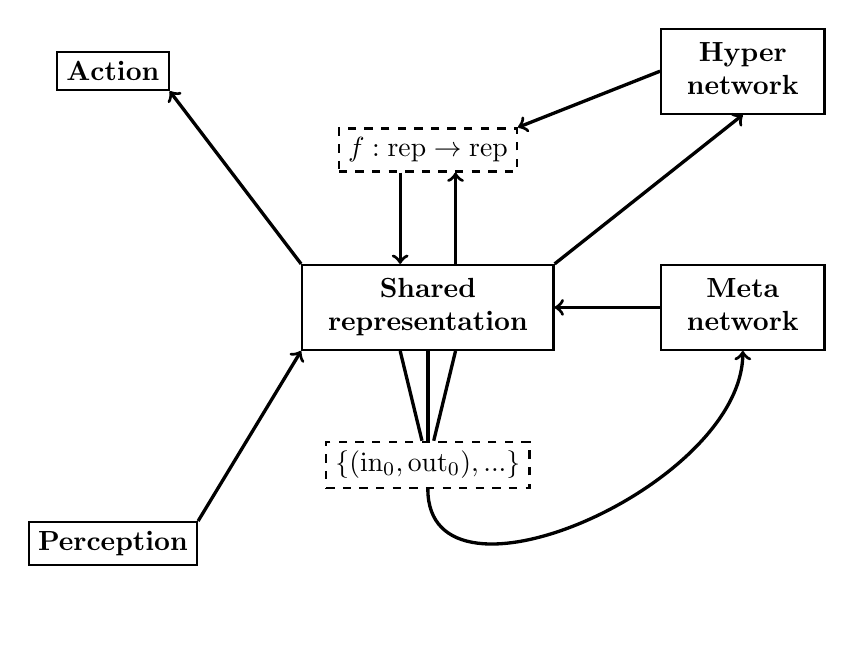
\begin{tikzpicture}[auto]

\node [draw, thick, align=center] at (0, 0) (rep) {\begin{tabular}{c}\textbf{Shared} \\ \textbf{representation}\end{tabular}};

% inputs, outputs


\node [draw, thick, align=center] at (-4, -3) (perc) {\textbf{Perception}};
\node [draw, thick, align=center] at (-4, 3) (act) {\textbf{Action}};
\path [draw, ->, very thick] (perc.north east) to (rep.south west);
\path [draw, ->, very thick] (rep.north west) to (act.south east);

% meta

\node [draw, thick, dashed, align=center] at (0, -2) (collection) {\(\{(\text{in}_0, \text{out}_0), ... \}\)};
\path [draw, very thick] (rep.south) to (collection);
\path [draw, very thick] ([xshift=-1em]rep.south) to (collection);
\path [draw, very thick] ([xshift=1em]rep.south) to (collection);

\node [draw, thick, align=center] at (4, 0) (meta) {\begin{tabular}{c}\textbf{Meta} \\ \textbf{network}\end{tabular}};
\path [draw, ->, very thick] (collection.south) to [out=-90, in=-90] (meta.south);
\path [draw, ->, very thick] (meta.west) to (rep.east);

% hyper

\node [draw, thick, align=center] at (4, 3) (hyper) {\begin{tabular}{c}\textbf{Hyper} \\ \textbf{network}\end{tabular}};
\node [draw, thick, dashed, align=center] at (0, 2) (transform) {\(f: \text{rep} \rightarrow \text{rep}\)};

\path [draw, ->, very thick] (rep.north east) to (hyper.south);
\path [draw, ->, very thick] (hyper.west) to (transform.north east);
\path [draw, ->, very thick] ([xshift=-1em]transform.south) to ([xshift=-1em]rep.north);
\path [draw, ->, very thick] ([xshift=1em]rep.north) to ([xshift=1em]transform.south);


\end{tikzpicture}
\end{figure}

\end{document}
